\documentclass[12pt]{article}
\usepackage[letterpaper, margin=1in]{geometry}
\usepackage{graphicx}
\usepackage{subcaption}
\graphicspath{{./Figures/}}
\usepackage{hyperref}
\usepackage{parskip}
\usepackage{amsmath}
%\allowdisplaybreaks % in case equations need to be broken across lines, probably should use align* with \stepcounter{equation}\tag{\theequation}\label{eq:7omegan} for equation numbering

\title{ELECENG 3CL4 Lab 2 Report}
\author{
    Aaron Pinto \\
    pintoa9 \\
    L02
    \and
    Raeed Hassan \\
    hassam41 \\
    L02
}

\begin{document}

\maketitle
\clearpage

\setcounter{section}{2}
\section*{Member Contributions}
Both group members contributed an even amount to both the exercises and the report. Both members went through the exercises together and contributed to all sections of the report.

\section*{Objective} % This is the brief description of the objective of the lab
The objective of this lab was to identify the plant model of a marginally-stable servomotor for the subsequent experiments.

\section{Perform Closed Loop Identification}
\subsection{Experiment 1: Time Domain Identification}
% iii) ran sim
% iv) K = 2
\begin{figure}[h!]
    \centering
    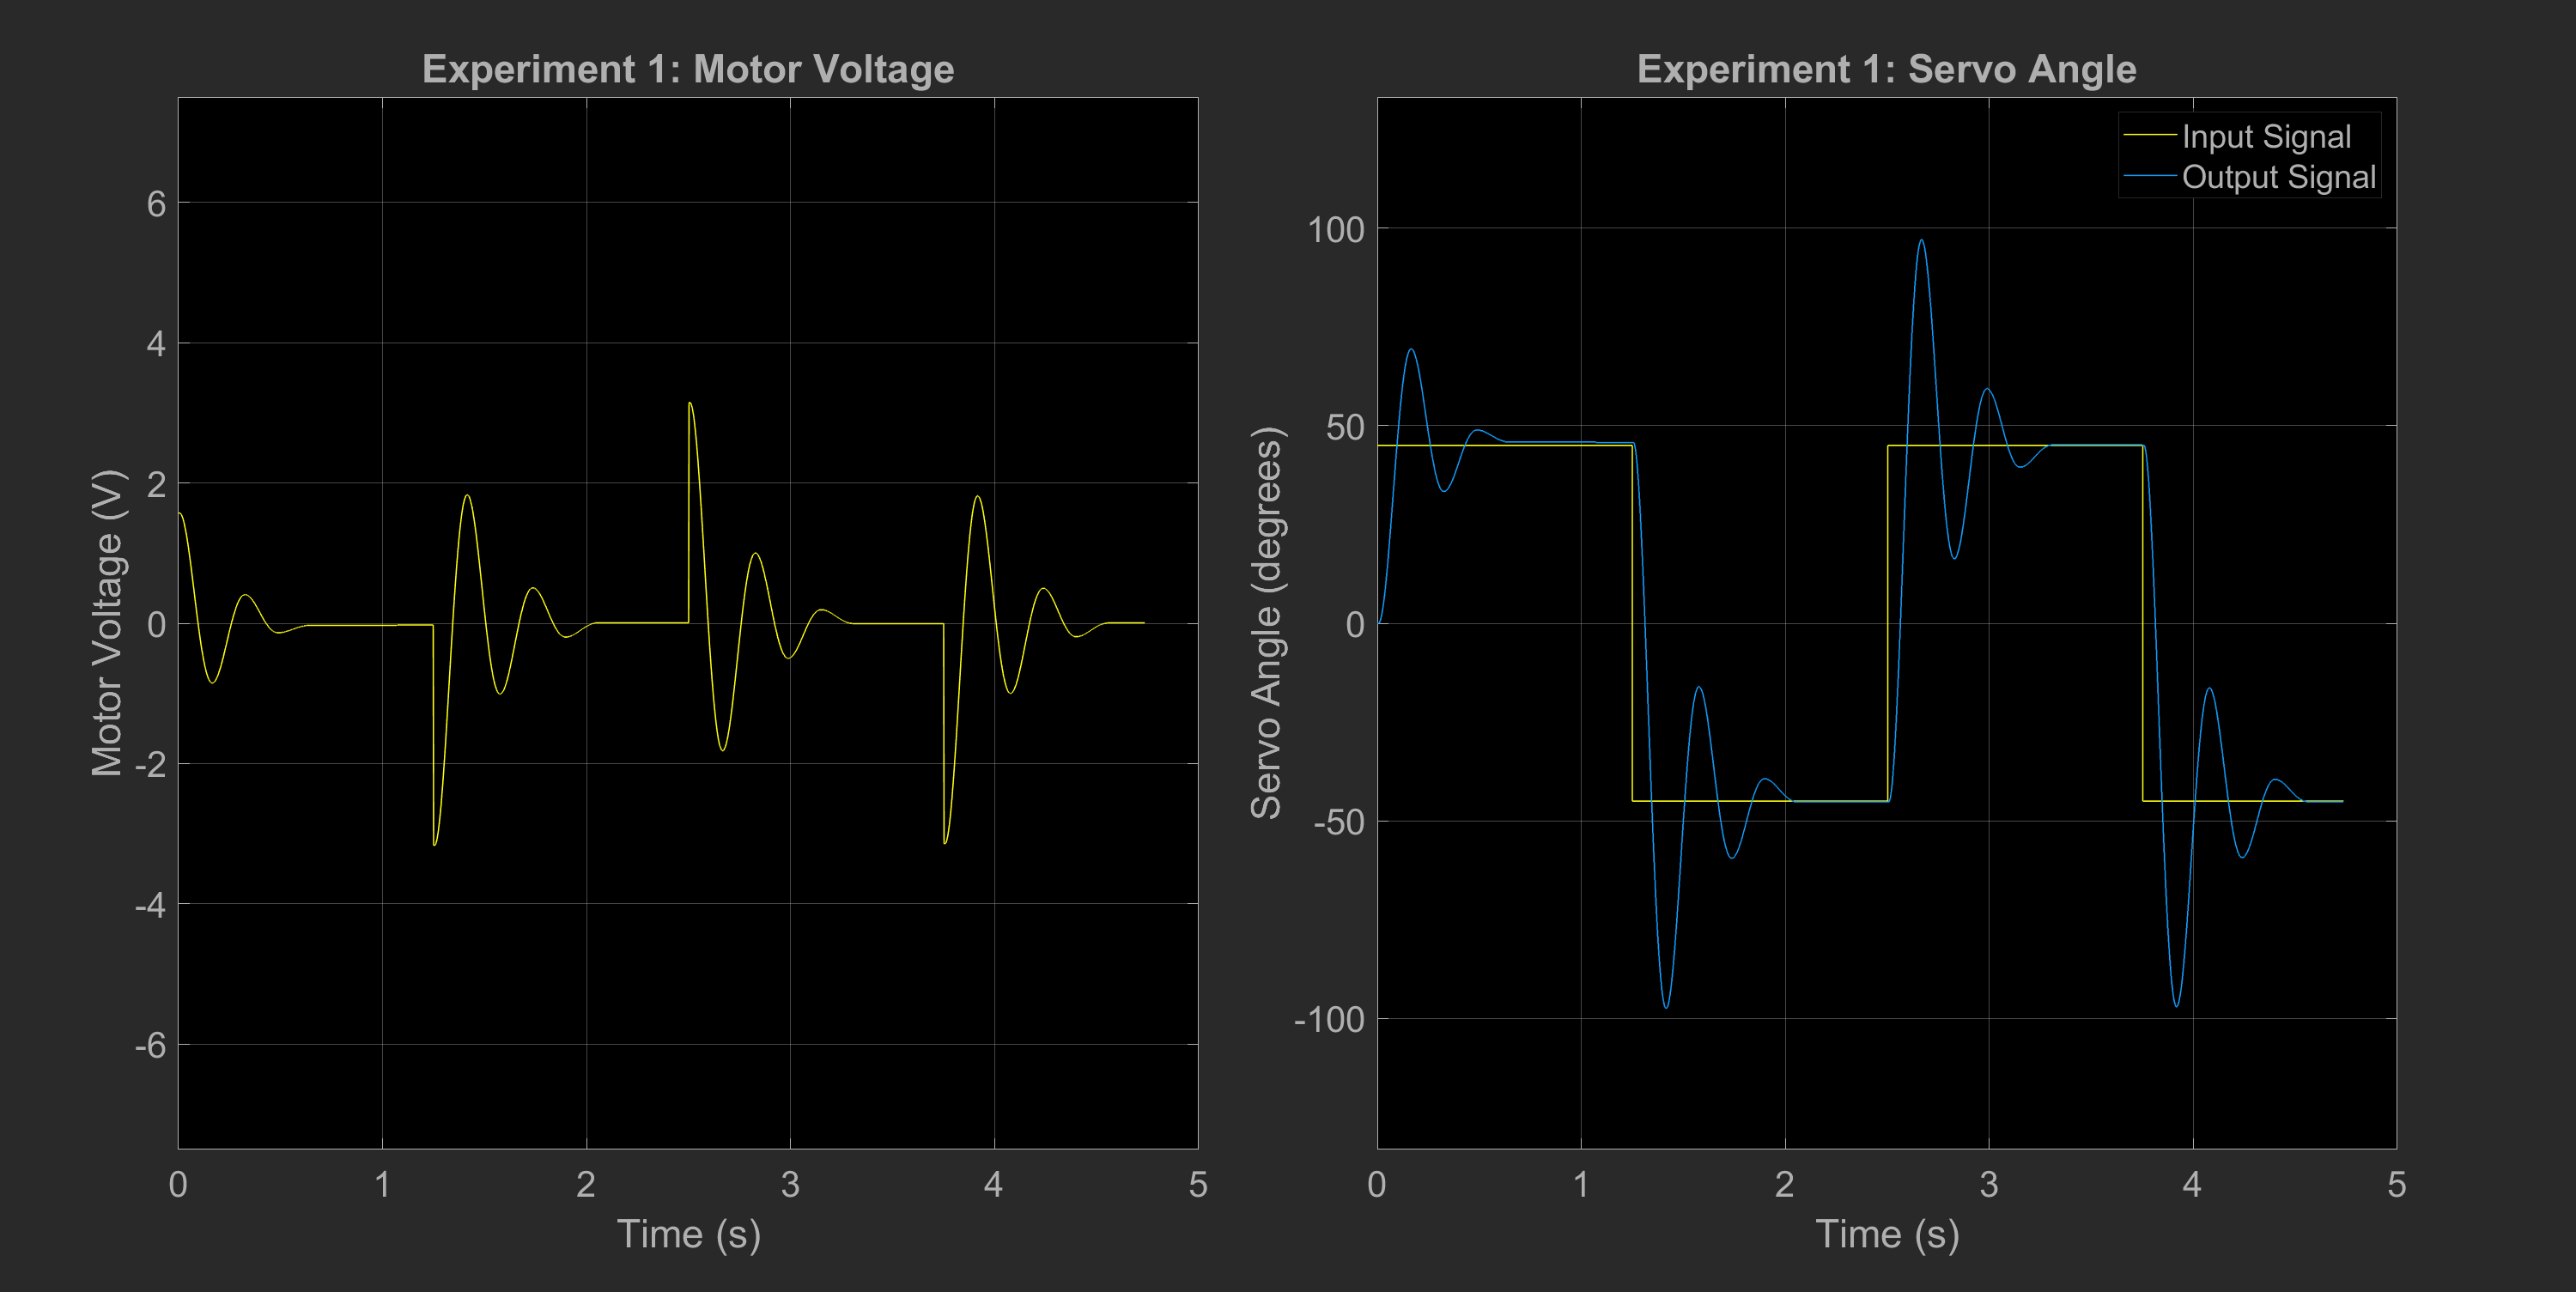
\includegraphics[width=\textwidth]{exp1}
    \caption{\label{fig:exp1}Motor Voltage and Servo Angle for Time Domain Identification}
\end{figure}
% v) measure height of first overshoot peak, time of first overshoot peak
% vi) measure the stuff
% vii) measure time difference from edge to time of first peak
% viii) record measurements
% ix) use measurements to calculate motor parameters

\subsection{Experiment 2: Frequency Domain Identification}
% vi) observe at 0.5 hz; small delay, some non-linear effects at direction change
\begin{figure}[h!]
    \centering
    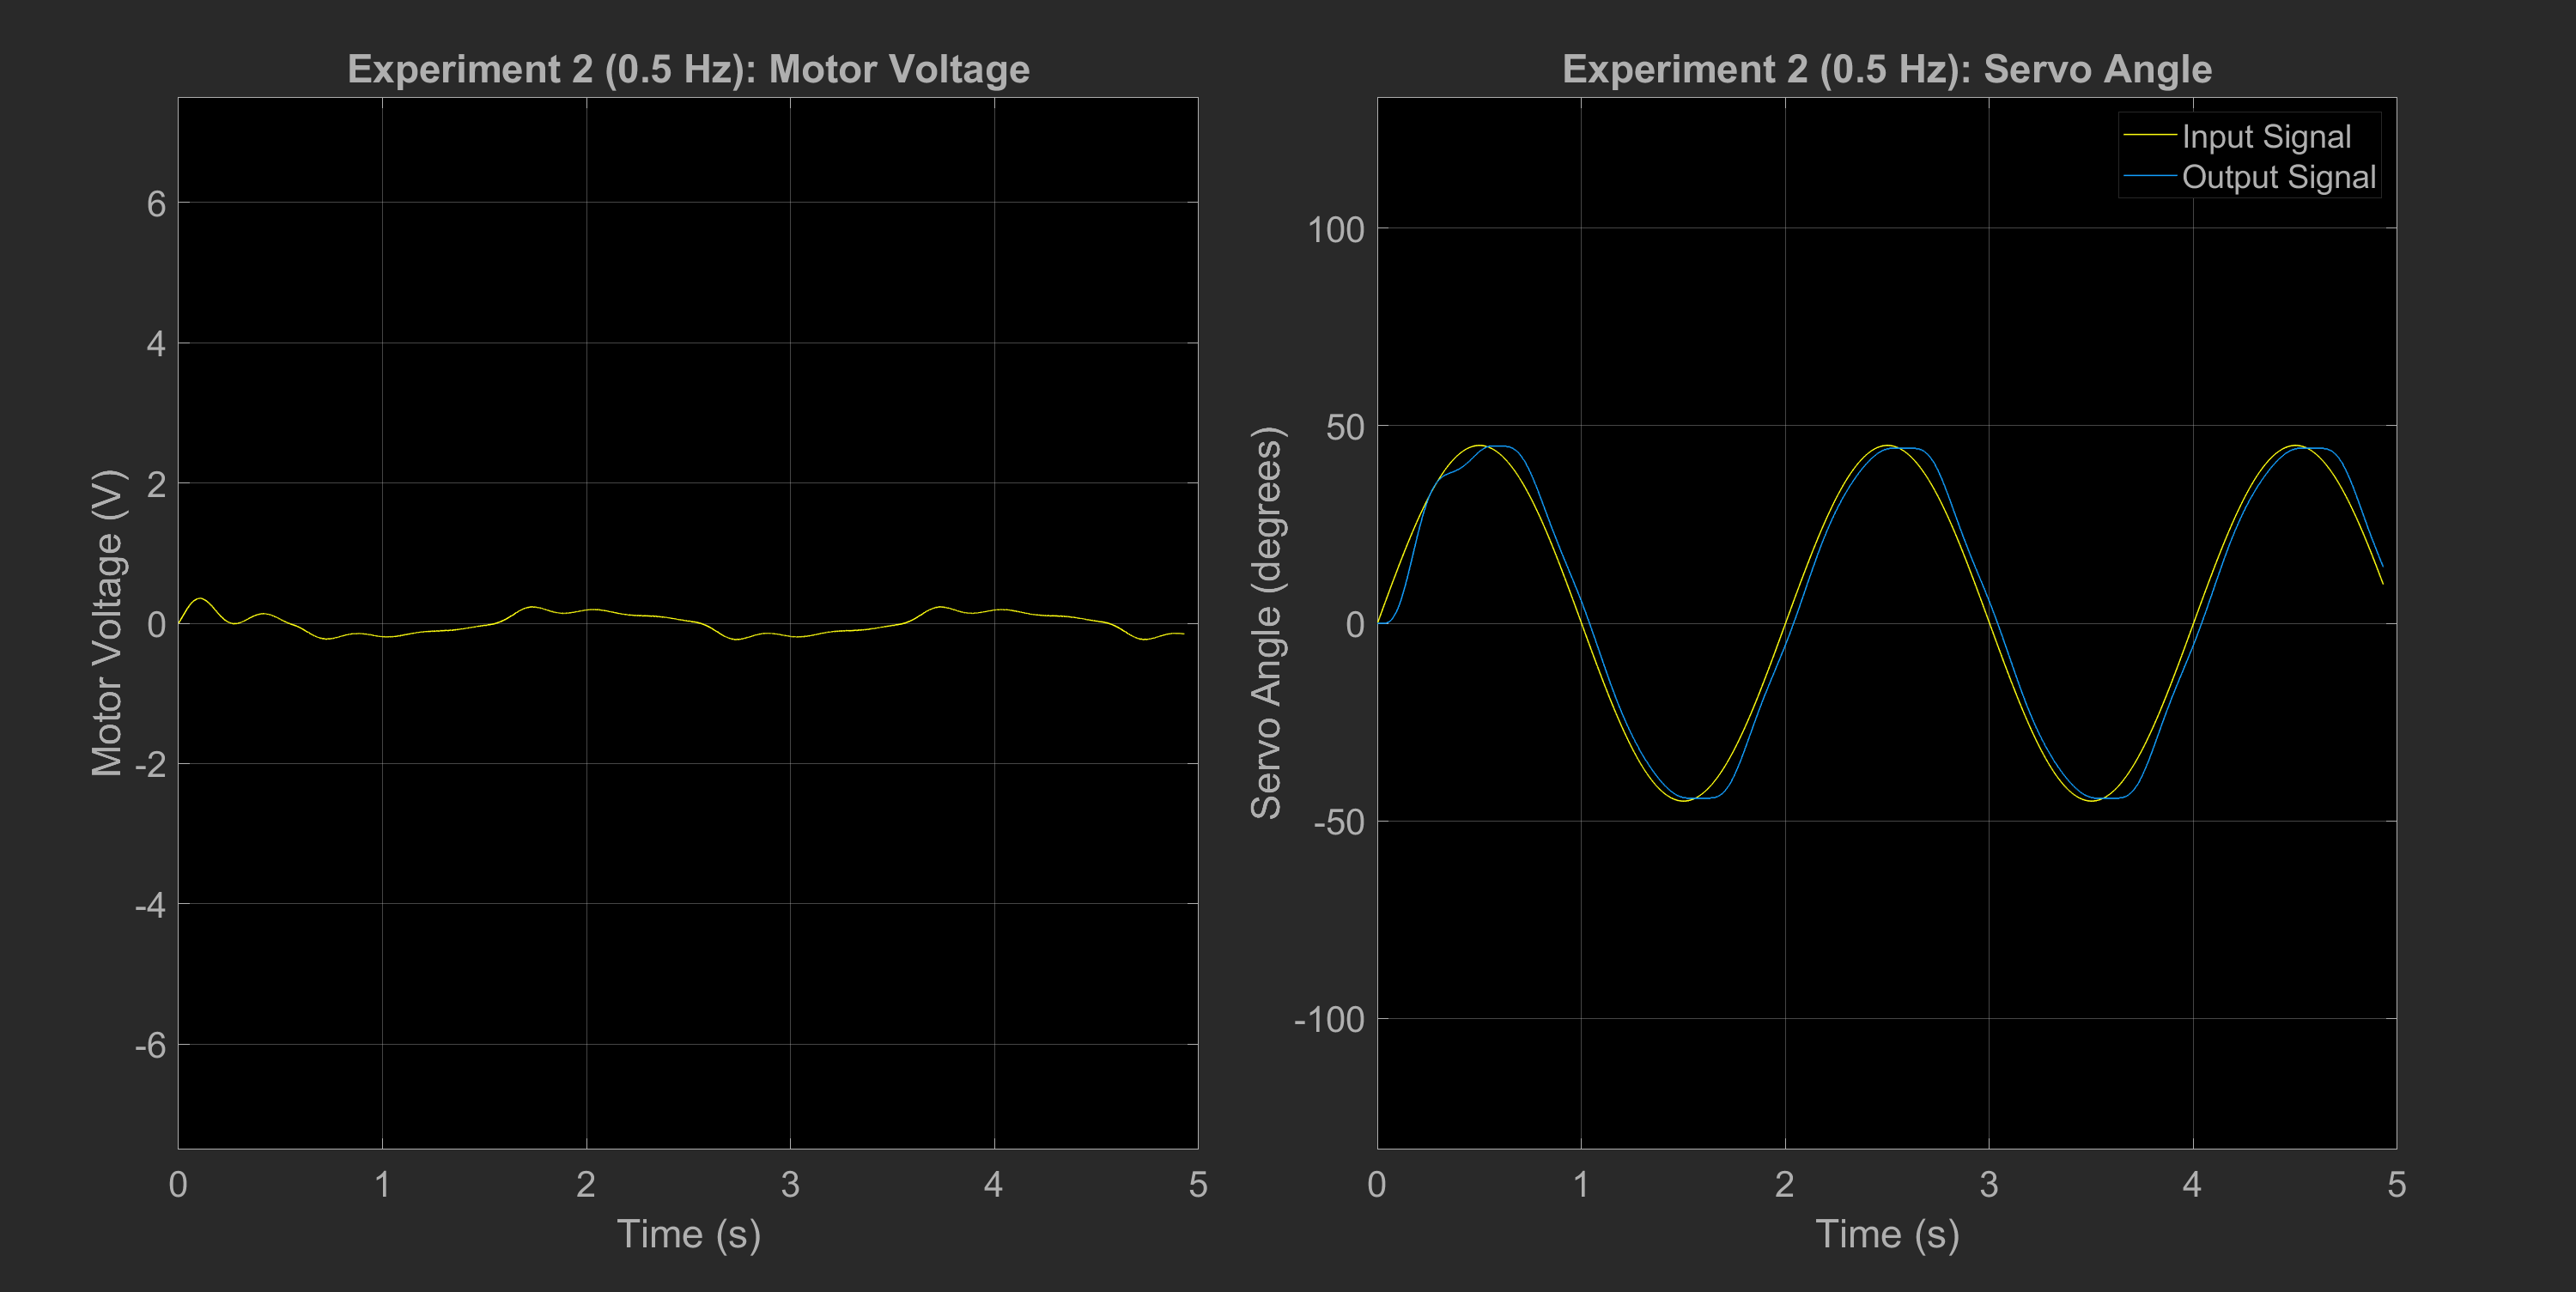
\includegraphics[width=\textwidth]{exp2_0.5}
    \caption{\label{fig:exp2_0.5}Motor Voltage and Servo Angle for 0.5 Hz Input Signal}
\end{figure}
% vii) 1 hz; slightly greater gain, slight longer delay, non-linear effects diminished
\begin{figure}[h!]
    \centering
    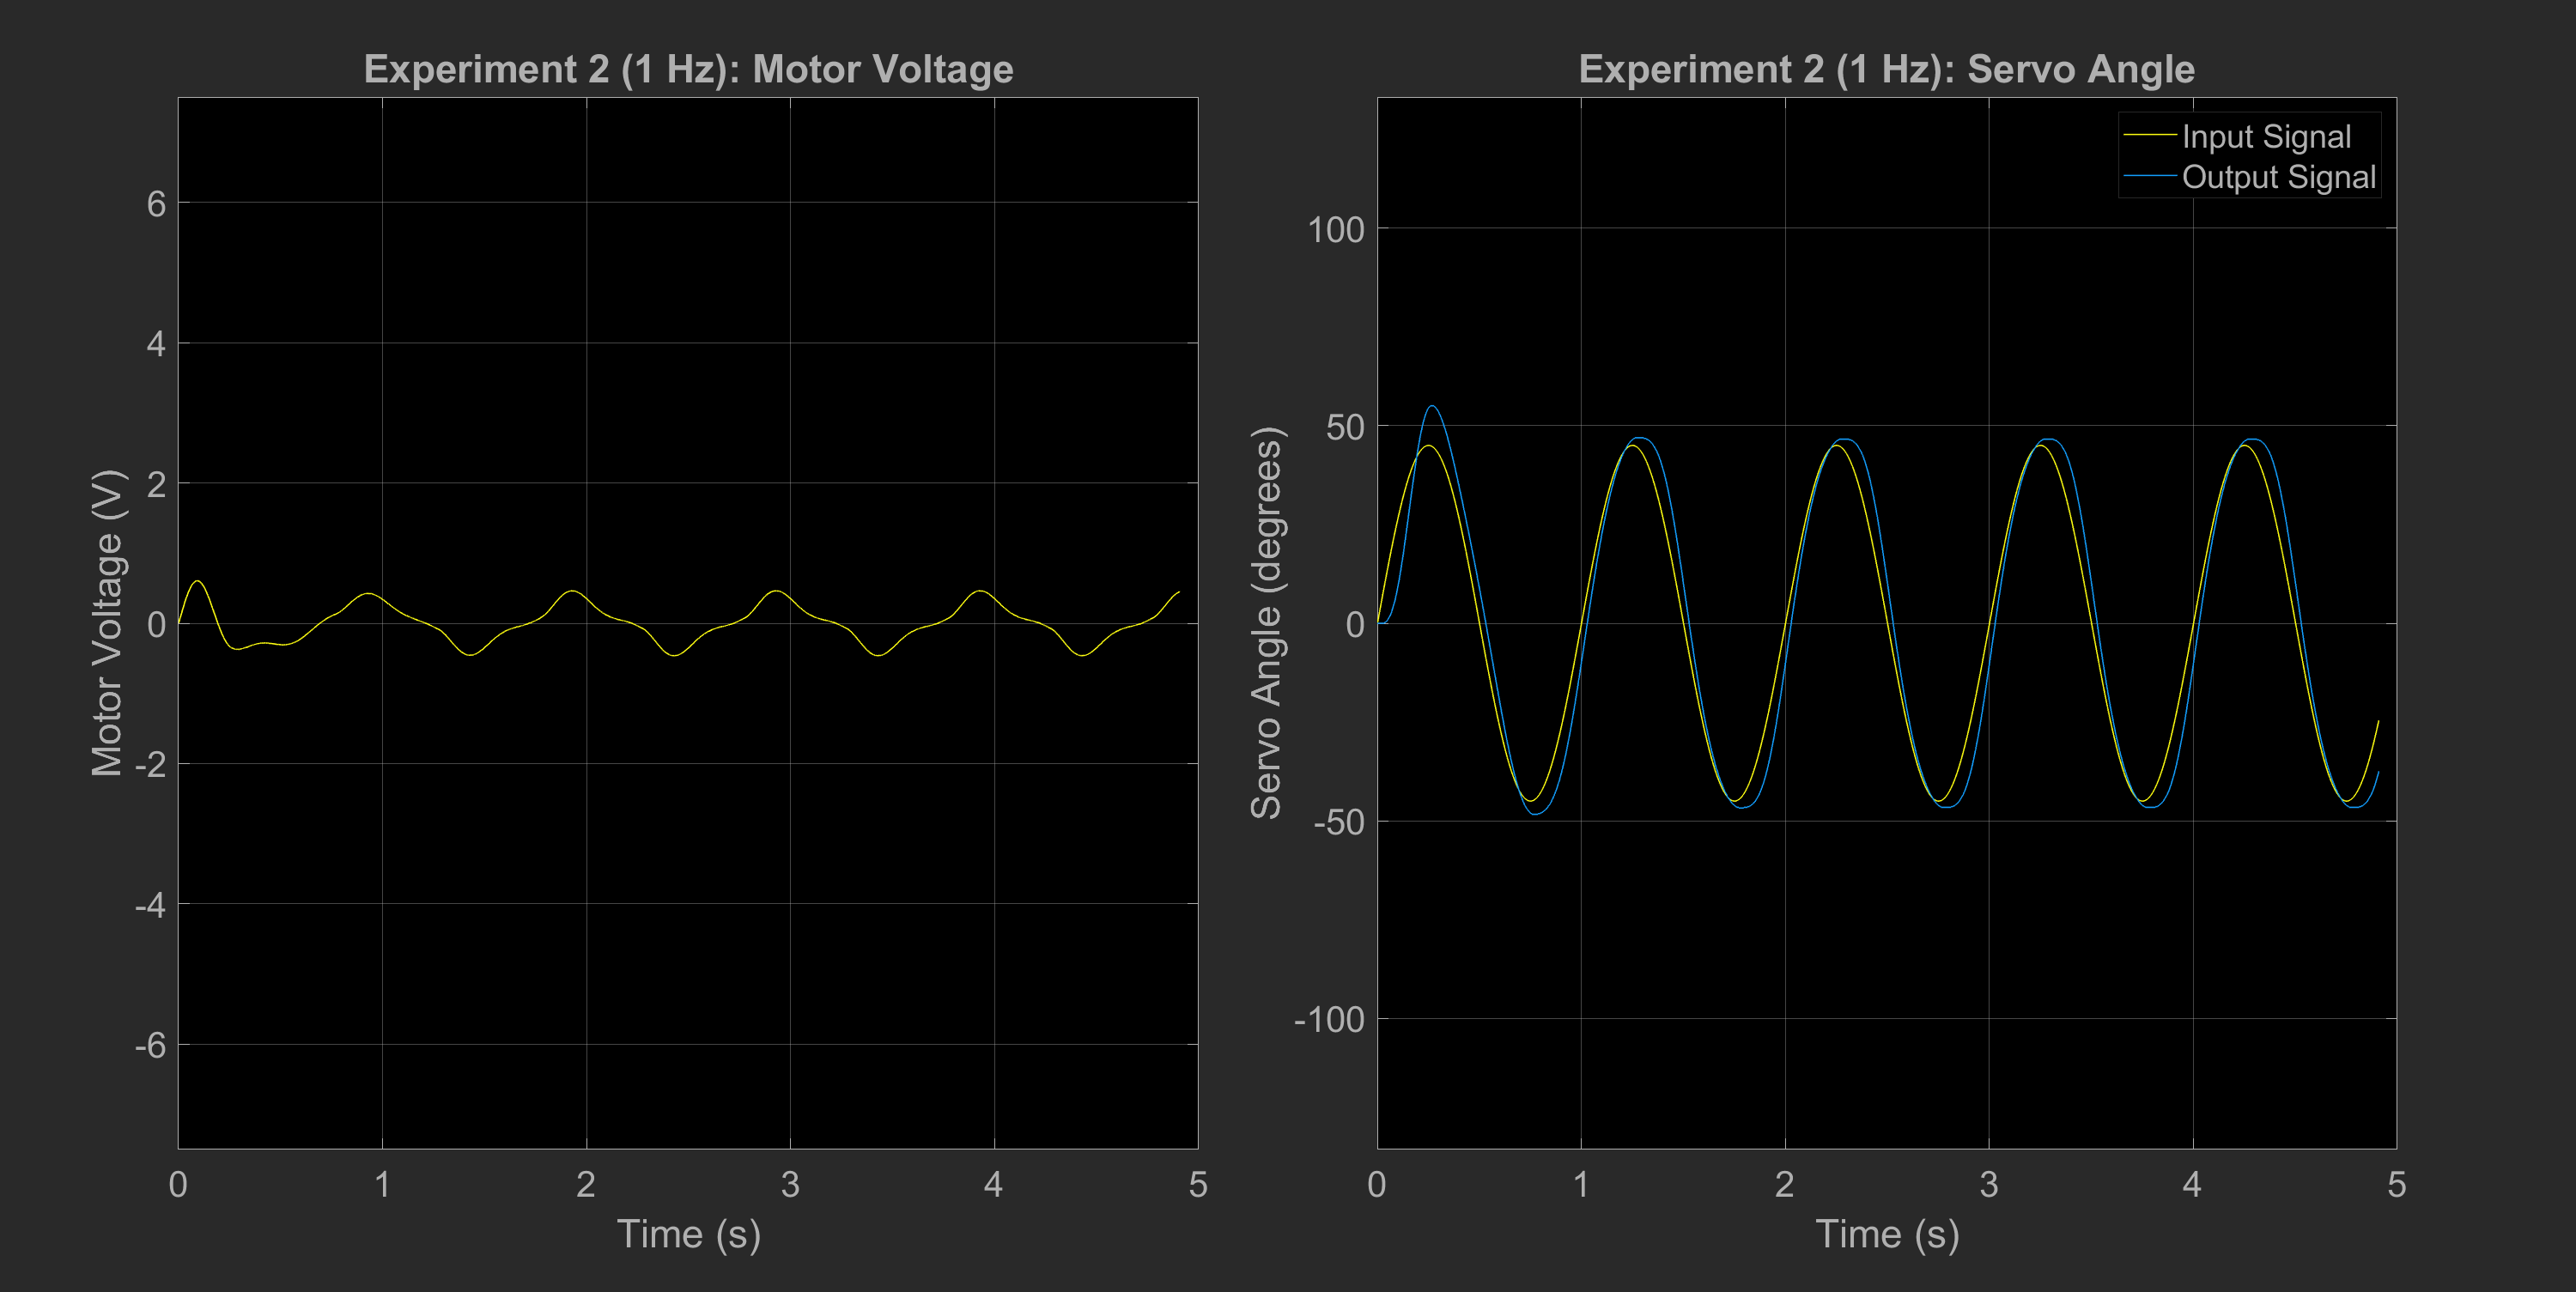
\includegraphics[width=\textwidth]{exp2_1}
    \caption{\label{fig:exp2_0.5}Motor Voltage and Servo Angle for 1 Hz Input Signal}
\end{figure}
% viii) 2 hz; gain signif greater, moderate delay, non-linear effects negligible
\begin{figure}[h!]
    \centering
    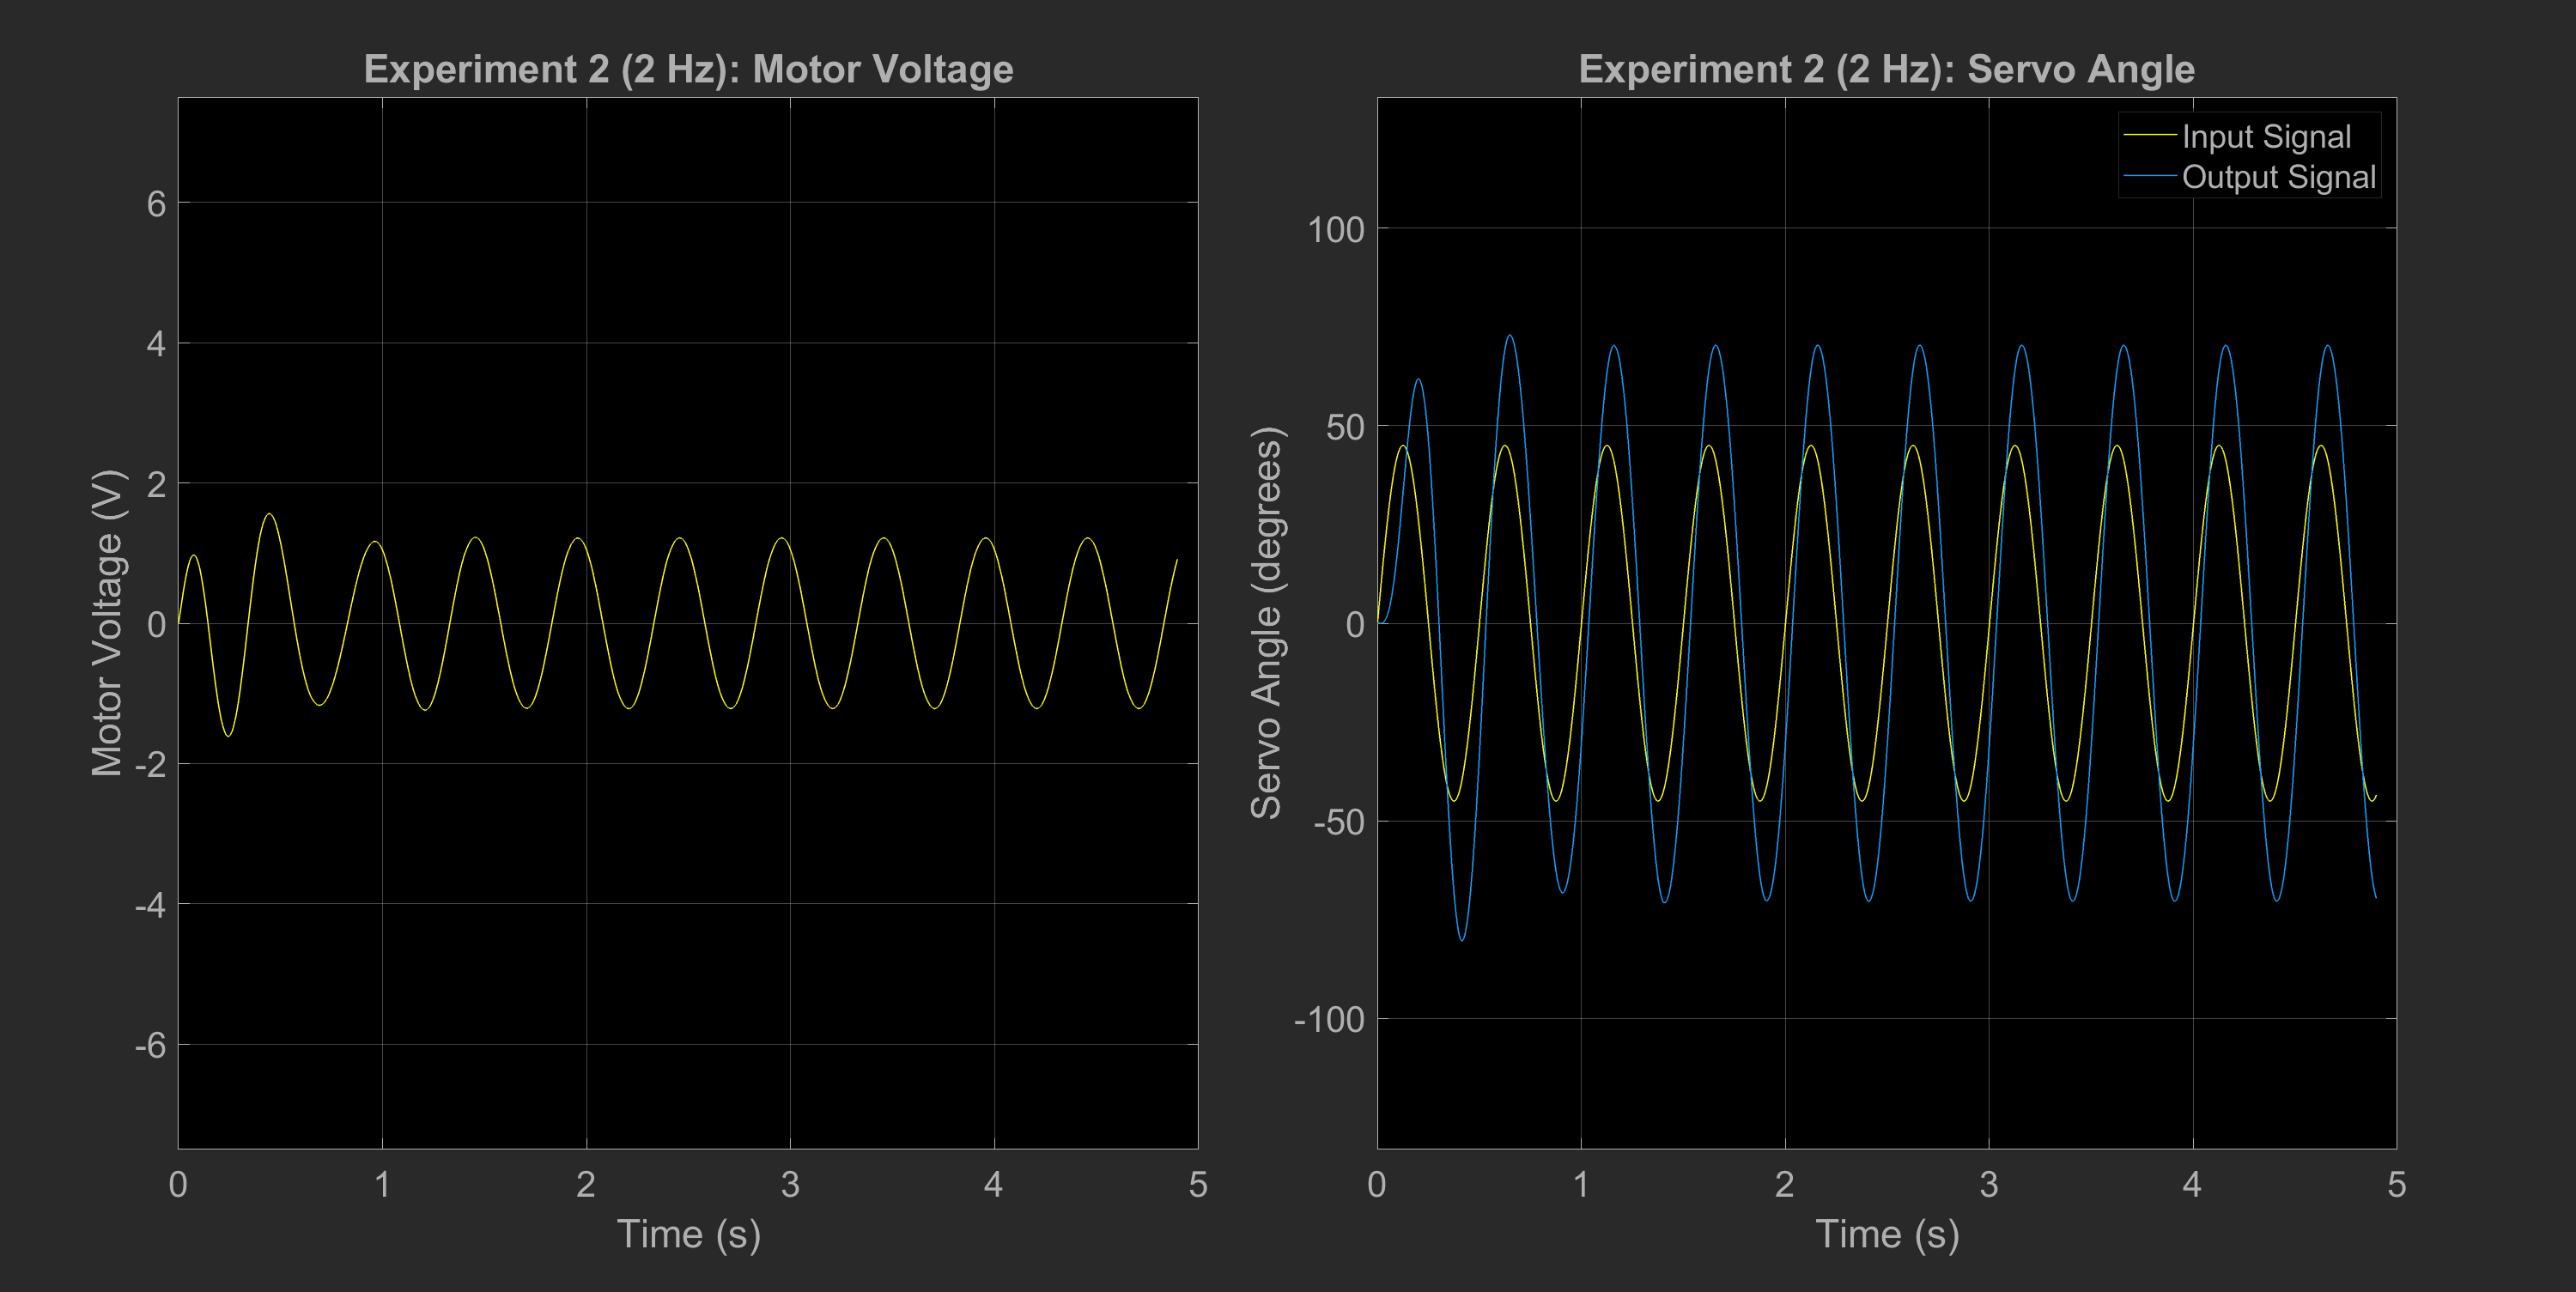
\includegraphics[width=\textwidth]{exp2_2}
    \caption{\label{fig:exp2_0.5}Motor Voltage and Servo Angle for 2 Hz Input Signal}
\end{figure}
% ix) 3 hz; gain signif greater, signifc delay, non-linear effects negligible
\begin{figure}[h!]
    \centering
    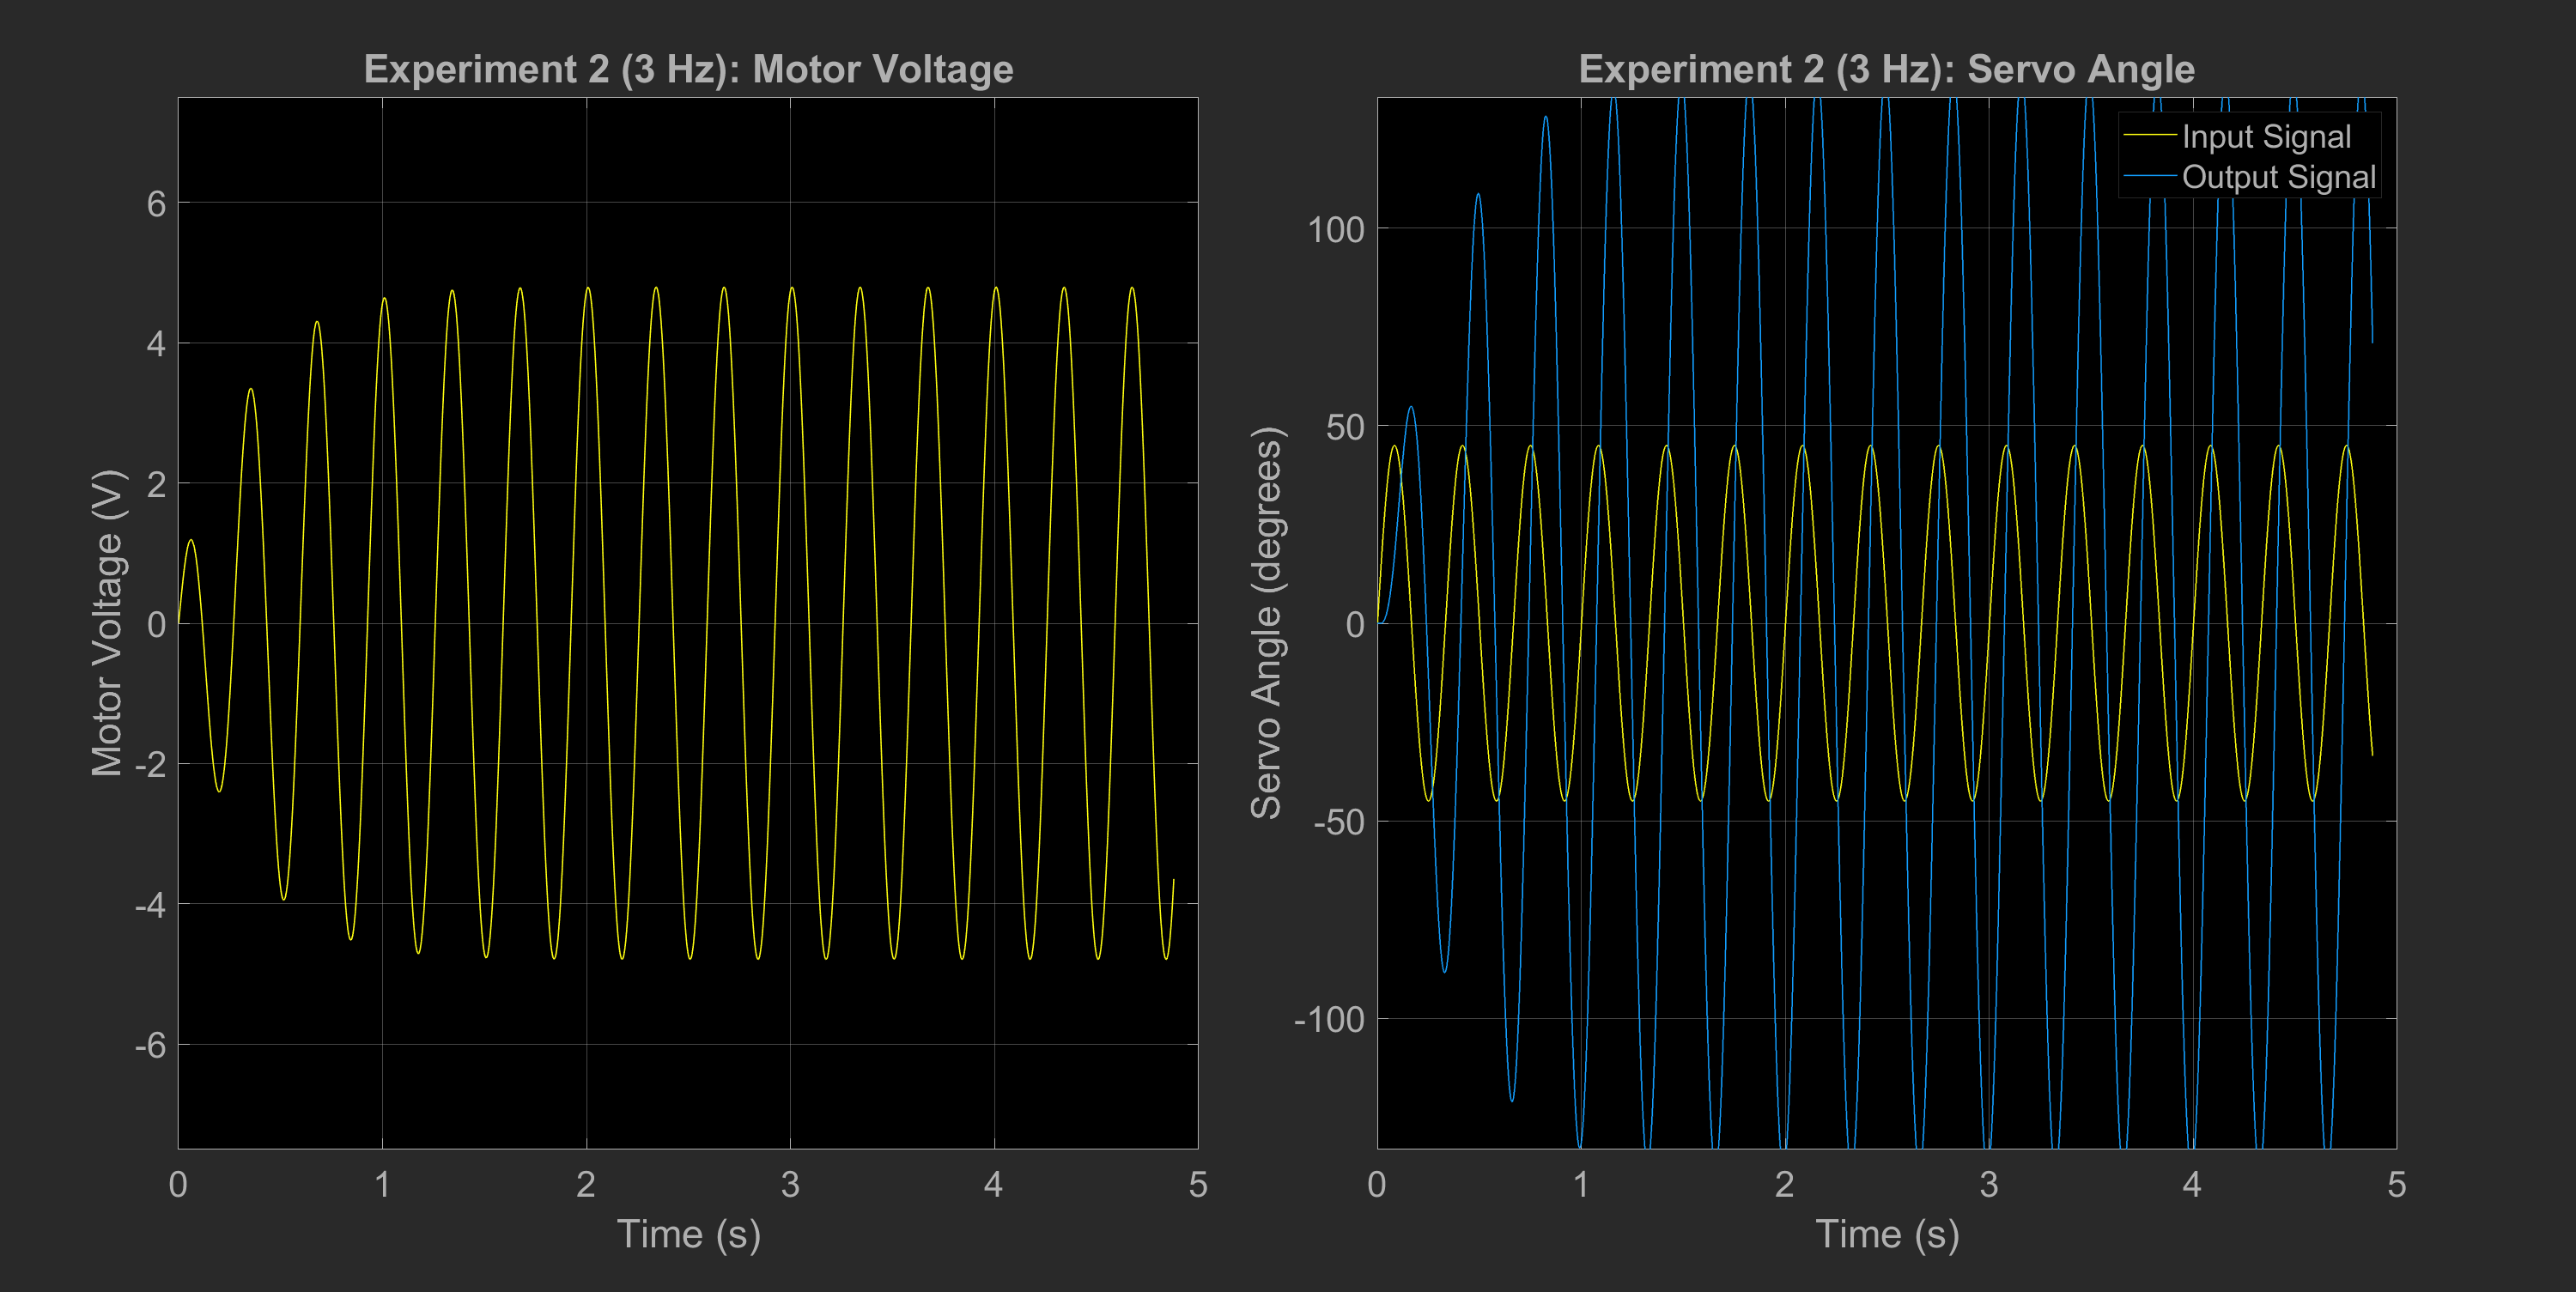
\includegraphics[width=\textwidth]{exp2_3}
    \caption{\label{fig:exp2_0.5}Motor Voltage and Servo Angle for 3 Hz Input Signal}
\end{figure}
% x) 4 hz; gain smaller than 3 hz, output almost completely out of phase w/ input
\begin{figure}[h!]
    \centering
    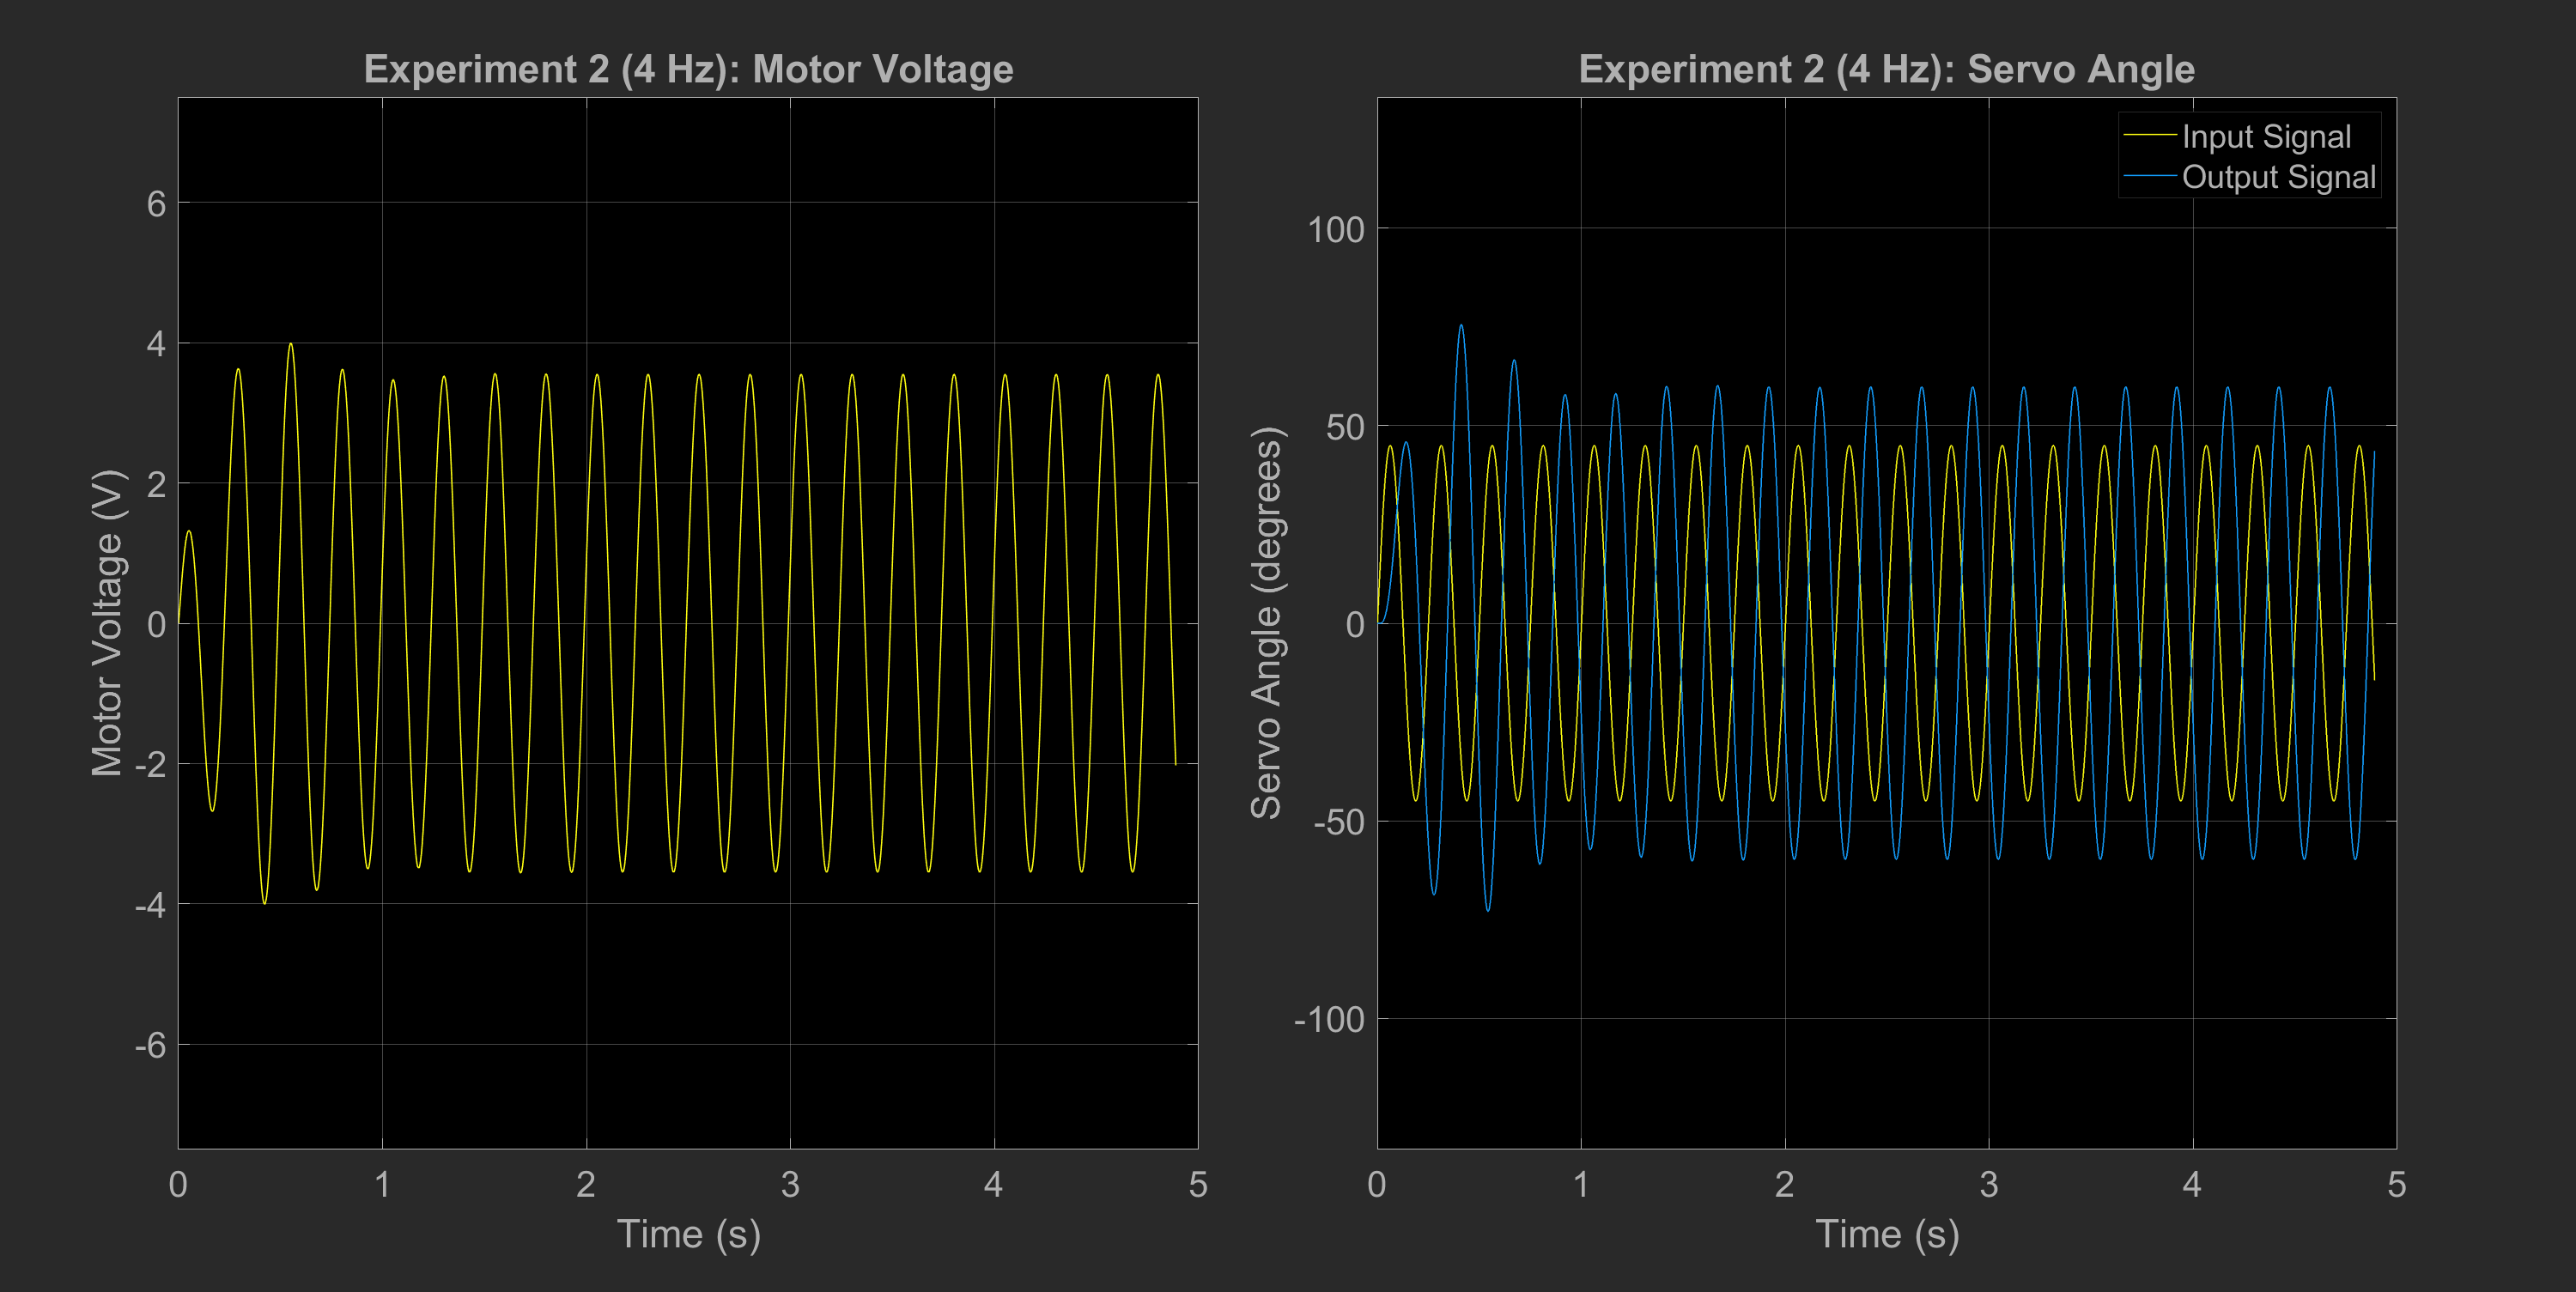
\includegraphics[width=\textwidth]{exp2_4}
    \caption{\label{fig:exp2_0.5}Motor Voltage and Servo Angle for 4 Hz Input Signal}
\end{figure}
% xi) 5 hz; 
\begin{figure}[h!]
    \centering
    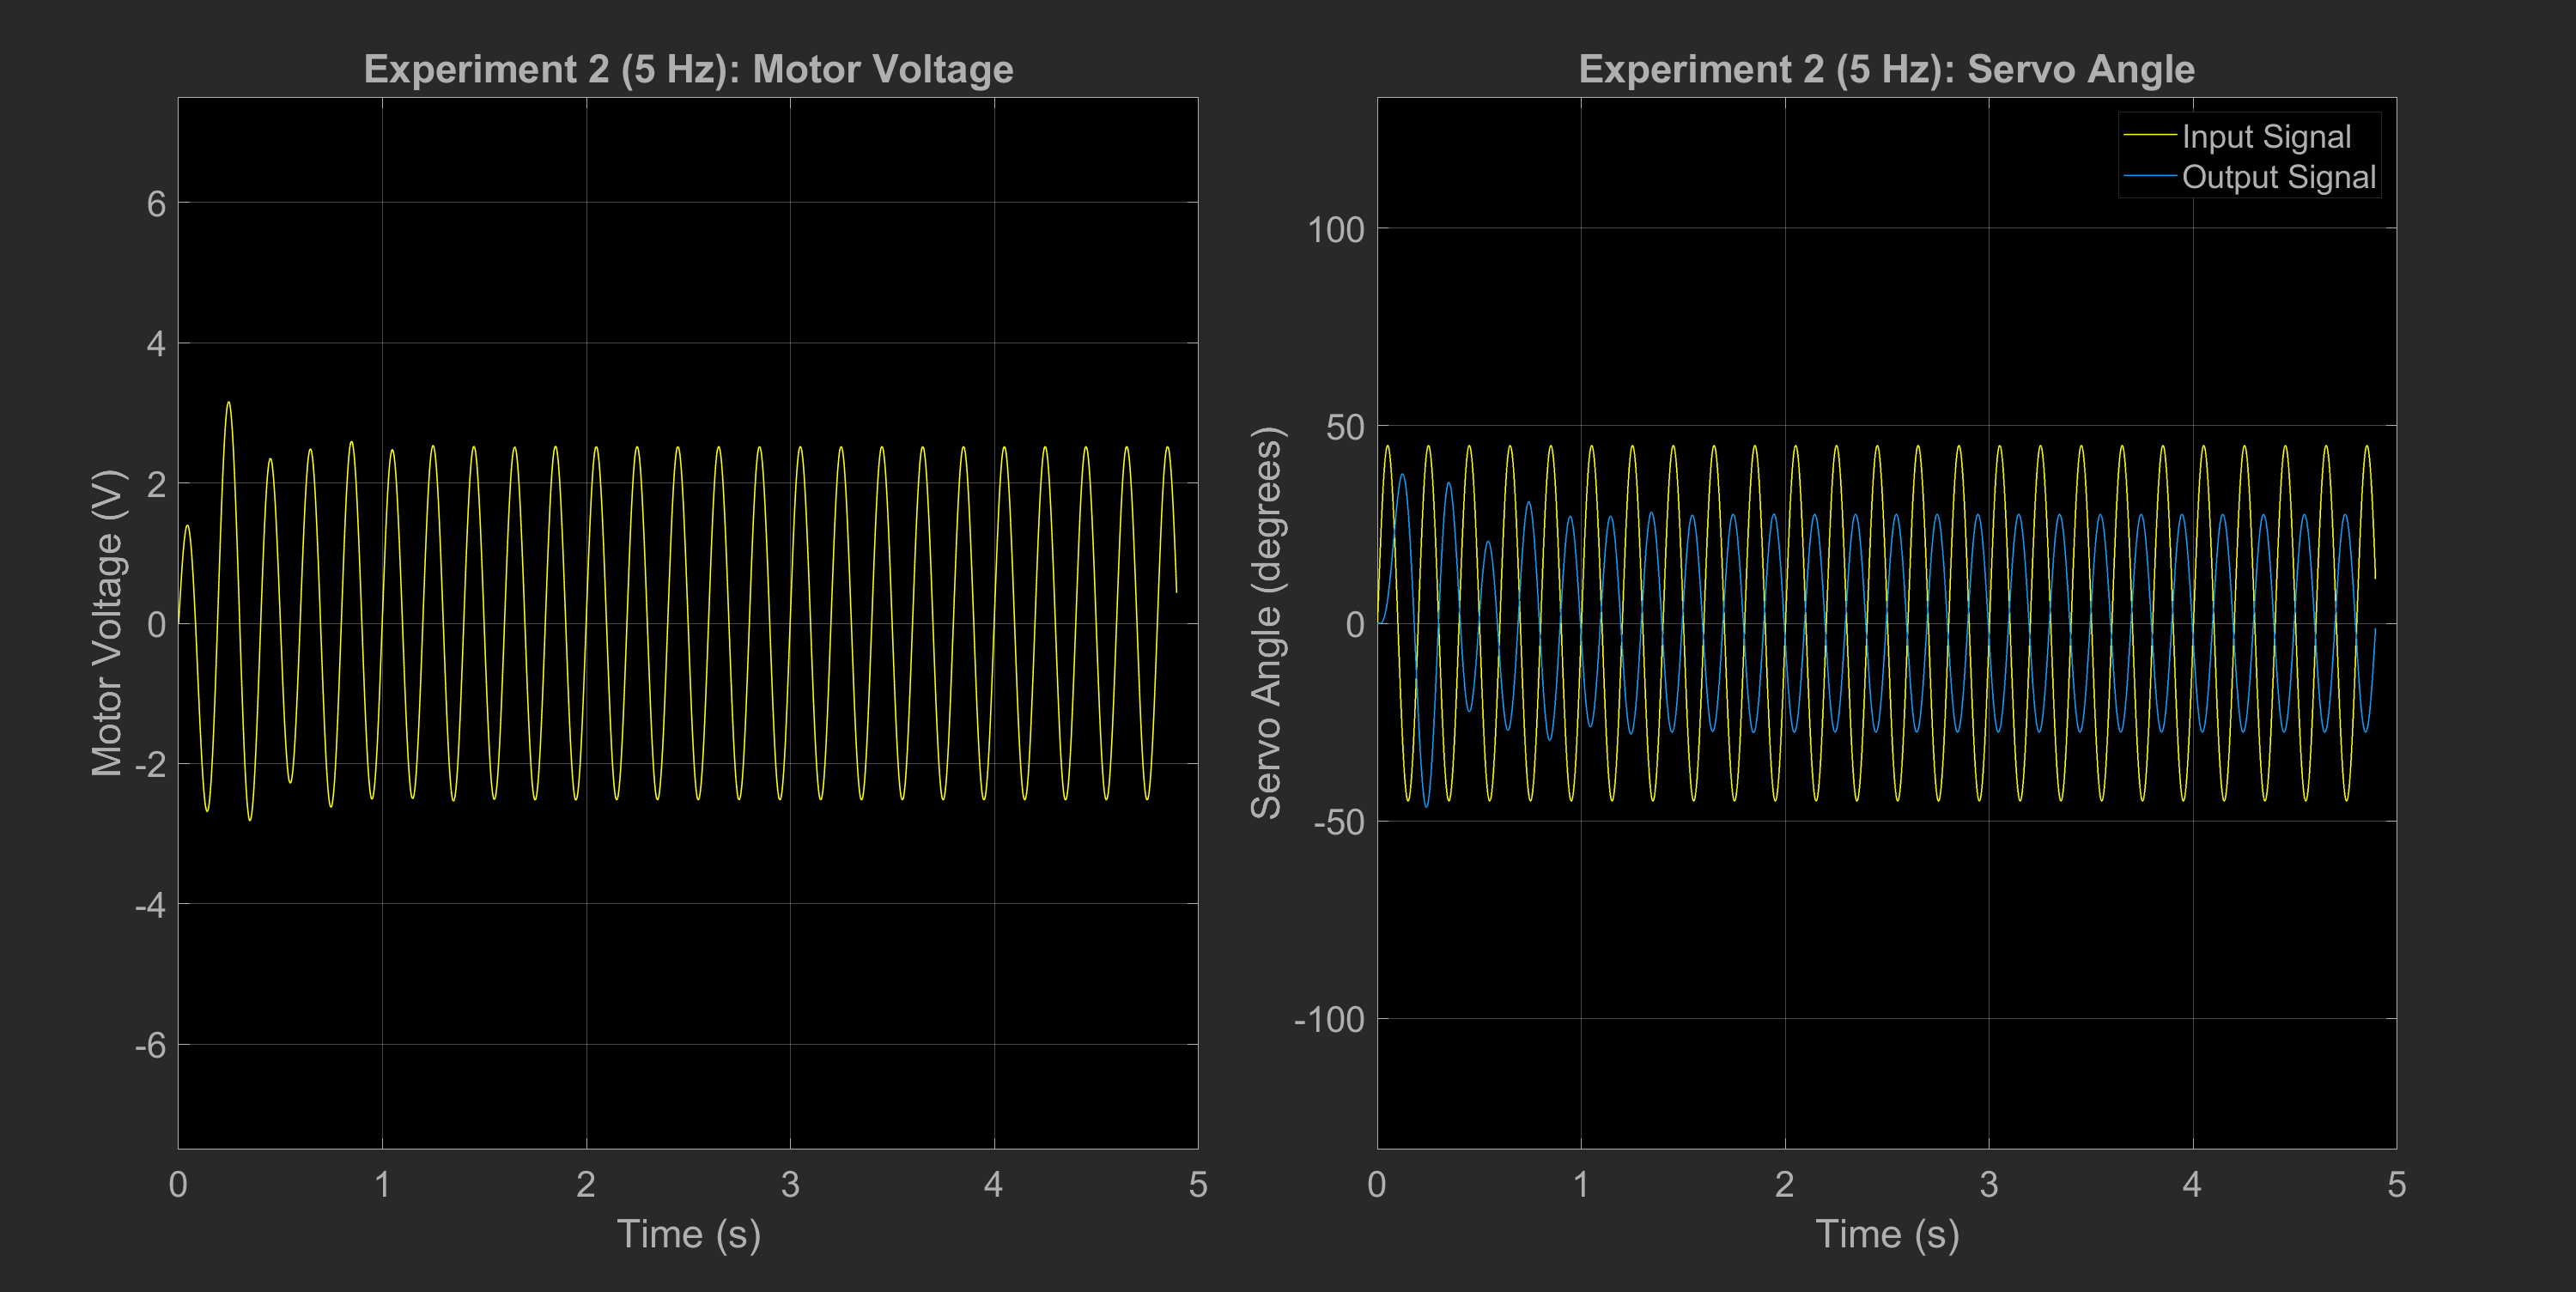
\includegraphics[width=\textwidth]{exp2_5}
    \caption{\label{fig:exp2_0.5}Motor Voltage and Servo Angle for 5 Hz Input Signal}
\end{figure}
% xii) 6 hz;
\begin{figure}[h!]
    \centering
    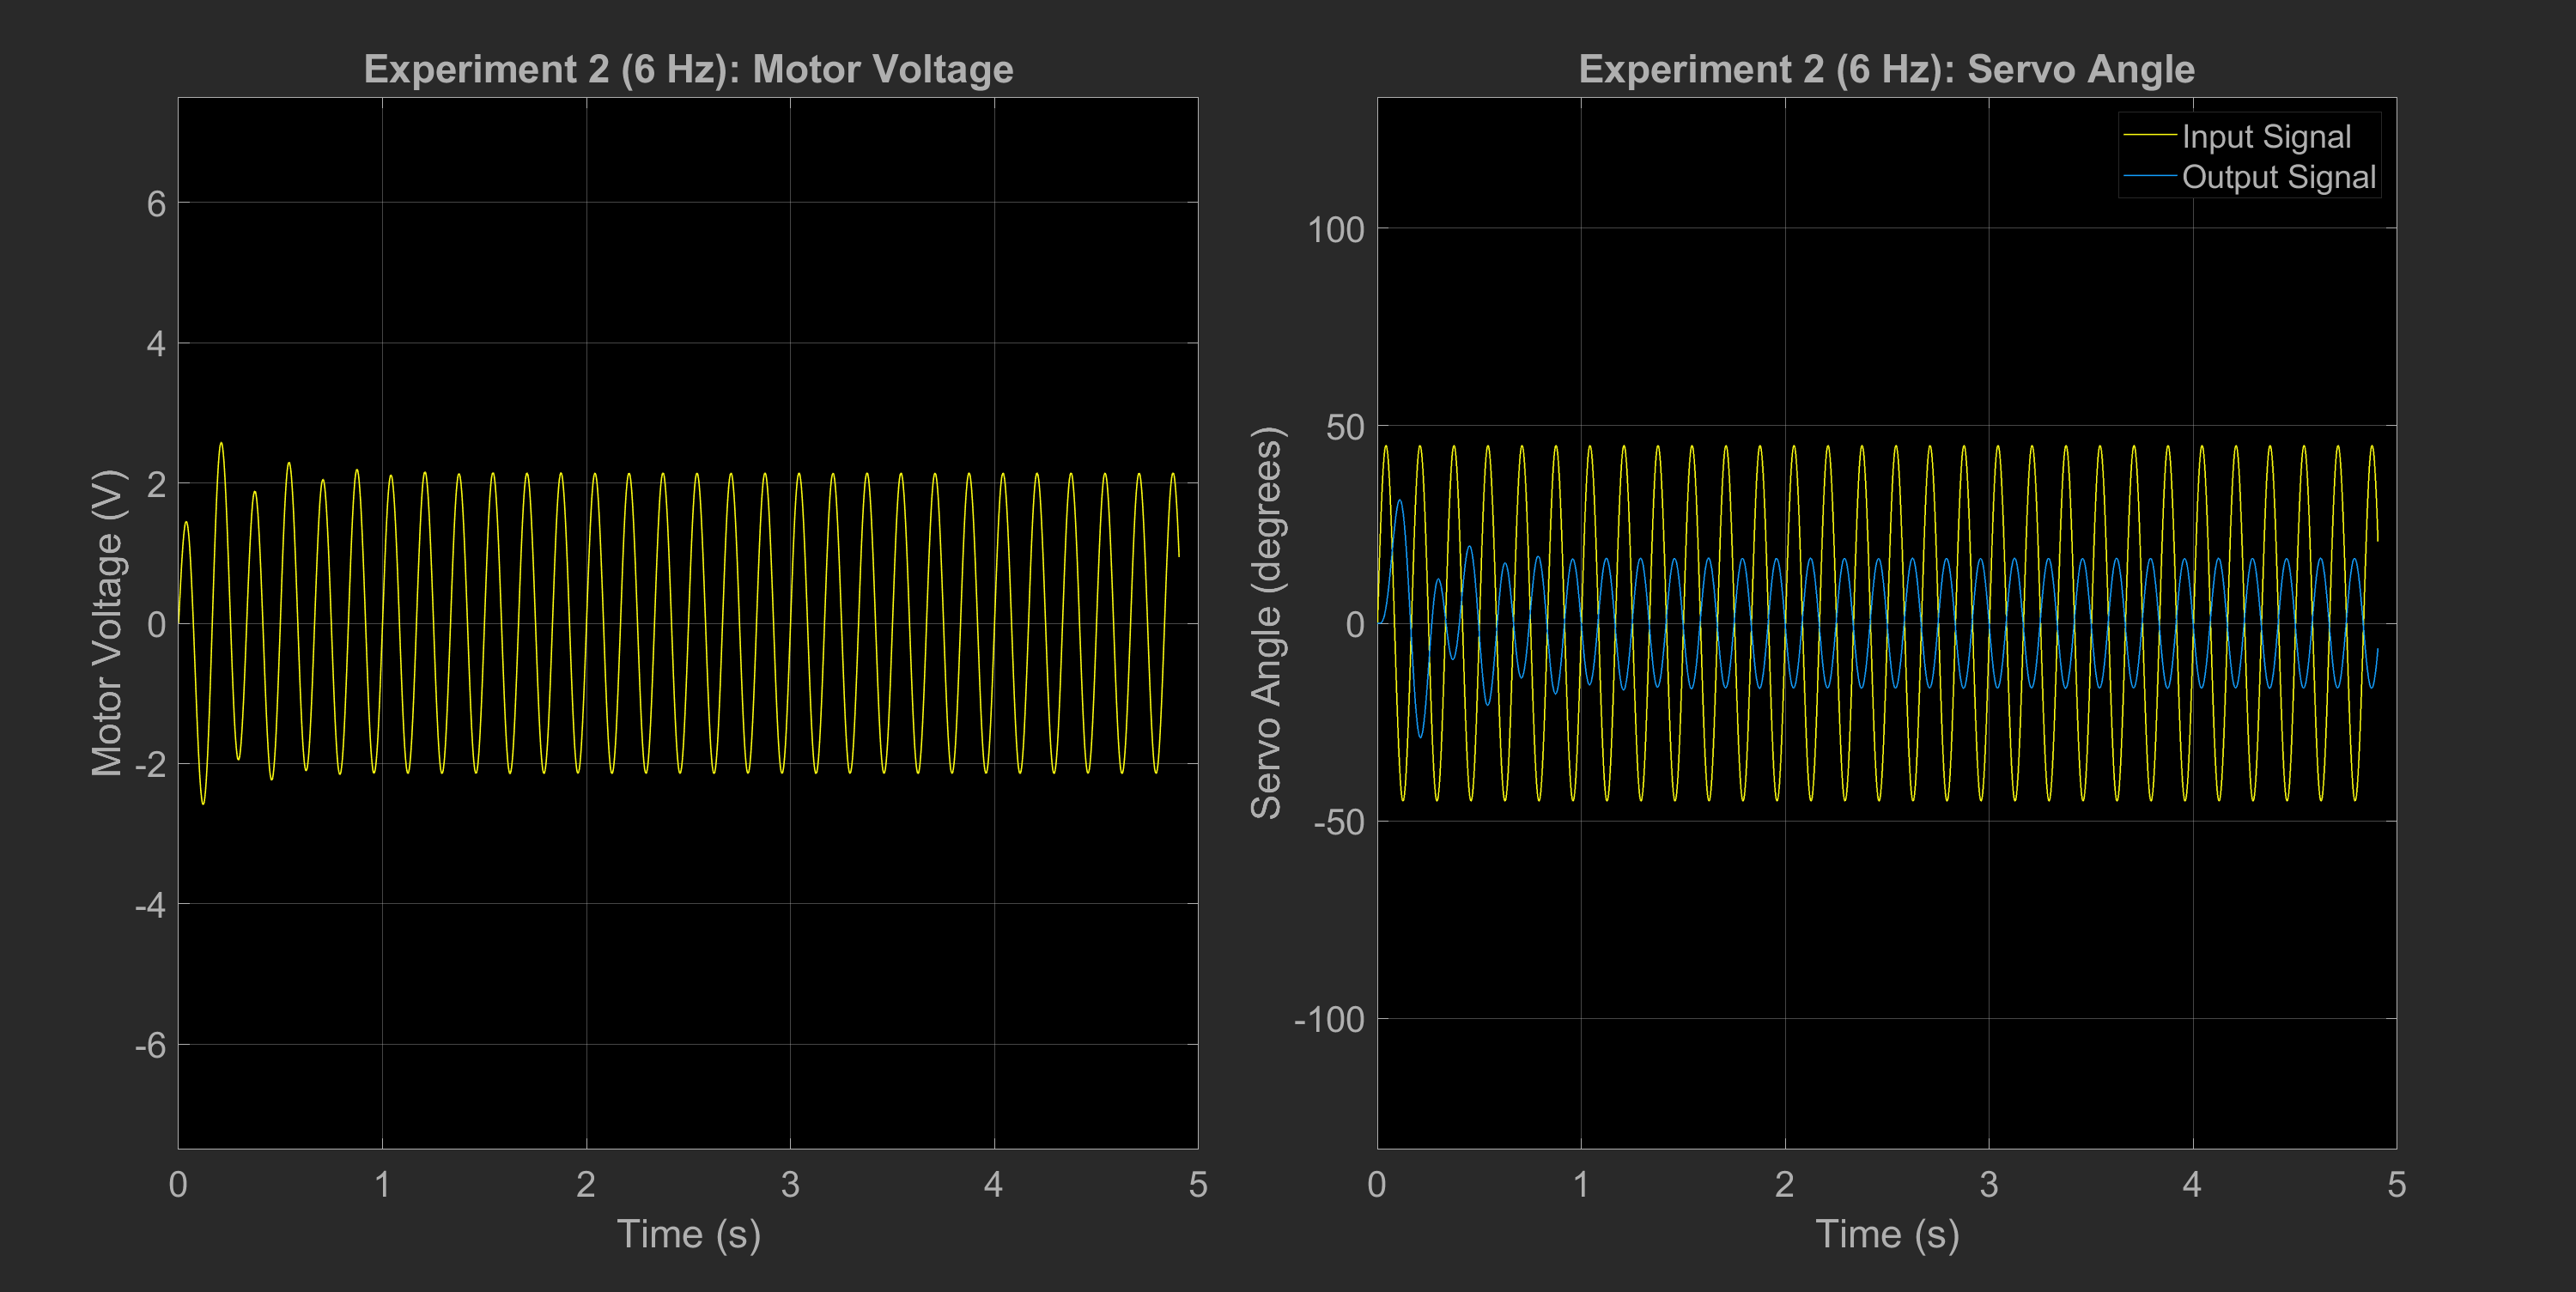
\includegraphics[width=\textwidth]{exp2_6}
    \caption{\label{fig:exp2_0.5}Motor Voltage and Servo Angle for 6 Hz Input Signal}
\end{figure}
% xiii) search for freq where mag reaches peak
% xiv) use measurements to calculate motor parameters
\clearpage

\section*{Comparison of Results and Discussion of Potential Discrepancies}
Our values for A and Tm were pretty close to each other using the 2 different methods. The discrepancies could've come from the non-linear effects of the motor or some shit xd.

\section*{Discussion on Improving the Accuracy of the Estimation of Model Parameters}
Who knows xd

\end{document}
